\documentclass[10pt,a4paper]{article}
\usepackage[utf8]{inputenc}
\usepackage[english]{babel}
\usepackage{amsmath}
\usepackage{amsfonts}
\usepackage{amssymb}
\usepackage{graphicx}
\usepackage{fullpage}
\usepackage{url}
\usepackage{caption}
\usepackage{subcaption}
\usepackage{float}
\author{Joan Puigcerver i Pérez\\
\begin{footnotesize}
\emph{joapuipe@upv.es}
\end{footnotesize}
}
\title{High Tide Prediction using Neural Networks}
\begin{document}
\maketitle
\section{Introduction}
In this work we present several neural network-based approaches to solve the problem of high tide prediction. This problem consists on, given an historical record of the tide heights, predict the tide height at some future point. This is useful to predict high tides, which are the result of climatic elements combined with stationary tidal systems specific for a particular area. The prediction of high tides has particular interest to anticipate climate disasters, like the one happened in Venice in 1966, when the Venice Lagoon rose by nearly 2 meters above the regular water level, causing damages valued in millions of Euros to homes, museums and other historical buildings.\\

The problem of tide prediction, or tide forecasting, is basically a time series prediction problem, which has been broadly studied in the literature and many approaches have been proposed to solve it, with relative success. Of course, the success of all these methods depend on the specific domain in which they are applied. For example, stock-market values prediction can be also modeled as a time series forecasting problem, but it has not been accurately modeled yet.\\

In the following sections, the explored neural networks architectures used to solve the tide prediction problem will be introduced, so as the experiments performed to compare them and, finally, the conclusions that can be extracted from these experiments.

\section{Neural Networks}
Two main neural network (NN) architectures have been compared: feed-forward neural networks (FFNN), and recurrent neural networks (RNN). It has been proved that NN, given the enough amount of parameters, can model the fitting of any function for a finite set of inputs, and time series prediction is basically a function fitting problem, where the output at time $t$ depends on the $D$ past output values (and optionally, also depends on other variables). The next equation formalizes this definition.

\begin{equation}
x_{t} = f(x_{t-1}, \ldots, x_{t-D})
\end{equation}

The key idea in this work is to model the unknown function $f$, with a neural network. So, the time series value $x_t$ is approximated by ($\theta$ are the parameters of the neural network, or more generally, the used model):
\begin{equation}
x_{t} \approx \hat{x}_t = f_\theta(x_{t-1}, \ldots, x_{t-D})
\end{equation}

\subsection{Feed-forward neural networks}
On of the basic architectures used for neural networks is the feed-forward architecture (FFNN). This architecture consists of an input layer, which has as many units as input variables the function to model has. Generally, each unit of a layer is connected to all units of the following layer. Feed-forward networks can consist only of the input and the output layers, but the set of functions that can be represented using this architecture is limited only to linear functions. However, by adding one or many non-linear \emph{hidden} layers between the input and the output layers, one can model any function behavior for a finite input set.\\

To solve the tide level prediction problem, we choose to predict the tide value at time step $t$, given the $D$ previous records of the water level. So, the input layer consists of $D$ units. The output unit uses a linear activation function, so, any real number can be approximated. The linear activation is given by equation \ref{eq:linear_act}. Vector $\mathbf{x}$ represents the input values to the unit from the previous layer and $\mathbf{w}$ the vector of weights associated to each input value. Both vectors have $N$ elements. In the case that a bias unit is used, it can be encoded as an extra dimension to the input of the unit, which a value equal to 1 for any input, and an additional dimension in the weights vector, encoding the bias term.\\

\begin{equation}\label{eq:linear_act}
g(\mathbf{x}) = \mathbf{x}^T \cdot \mathbf{w} = \sum_{i=1}^N x_i w_i
\end{equation}

We used several hidden layers with different number of units for each layer. Each unit of the hidden layer is activated by a sigmoid function, which is defined by equation \ref{eq:sigmoid_act}. Again, a bias term can be introduced as explained before.\\

\begin{equation}\label{eq:sigmoid_act}
g(\mathbf{x}) = \frac{1}{1 + e^{-\mathbf{x}^T \cdot \mathbf{w}}}
\end{equation}

Figure \ref{fig:ffnn} shows the graphical representation of the best feed-forward network found on the performed experiments. The neural network is composed by two hidden layers. It uses the past 24 hours records ($D$) to predict the next record. The number of hidden units in each hidden layer is 20.\\

\subsection{Recurrent neural networks}
A simple recurrent neural network architecture derived from the Elman architecture have been used. The basic Elman network consists of one hidden layer with recurrent connections to itself, so the inputs of the hidden layer are the outputs of the input layer and the previous state of the hidden layer. We extended this architecture to consider not only the last state of the hidden layer, but the past $P$ states of the hidden layer. In the case of multilayer recurrent neural networks, all the hidden layers have this recurrent connection. The output units have the same activation function as before. The activation of the hidden units is also a sigmoid function.\\
%, but the input depends not only on the input from the previous layer $\mathbf{x}$, but also on the last $P$ outputs of the hidden layer: $\mathbf{s}_{t-1}, \ldots, \mathbf{s}_{t-P}$.

%\begin{equation}
%f(\mathbf{x},\mathbf{s}_{t-1}, \ldots, \mathbf{s}_{t-P}) = \frac{1}{1 + e^{-(\mathbf{x}^T \cdot \mathbf{w} + \sum_{i=1}^P \mathbf{s}_{t-i}^T \cdot \mathbf{v}_{t-i} )} }
%\end{equation}

Figure \ref{fig:rnn} shows the graphical representation of the best found recurrent neural network on the performed experiments. Each hidden layer uses its two last outputs ($P$) in a recurrent connection.

\begin{figure}[h]
\centering
\begin{subfigure}[b]{0.7\textwidth}
\centering
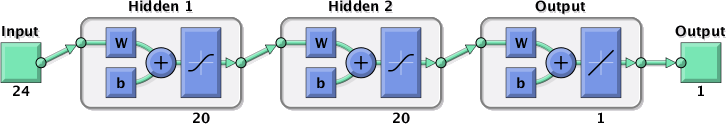
\includegraphics[width=\textwidth]{ffnn_win.png}
\caption{Feed-forward neural network}
\label{fig:ffnn}
\end{subfigure}
\\
\begin{subfigure}[b]{0.7\textwidth}
\centering
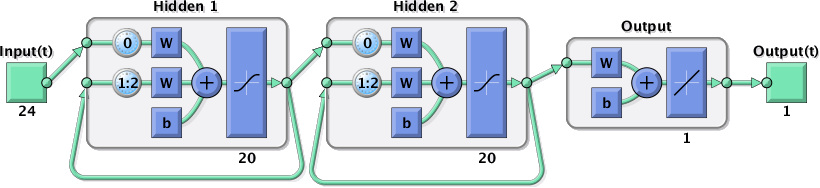
\includegraphics[width=\textwidth]{rnn_win.png}
\caption{Recurrent neural network}
\label{fig:rnn}
\end{subfigure}
\caption{The best feed-forward and recurrent neural network architectures found during the experimentation. Both use the previous 24 records to predict the next one and both have two hidden layers with 20 units in each of them. The hidden layers of the recurrent network use their last two hidden states.}
\end{figure}

\section{Experiments}
MATLAB Neural Network Toolkit was used to make the comparison among different architectures. Both feed-forward and recurrent neural networks are trained using Levenberg--Marquardt algorithm (LMA)\cite{more1978levenberg,hagan1994training}, an optimization algorithm that interpolates between the Gauss--Newton algorithm and gradient descent. This method showed a faster convergence than the usual gradient descent backpropagation algorithm, which is the standard one used for neural networks learning. In the case of recurrent neural networks, the network is unfolded using the backpropagation trough time (BPTT) method\cite{mozer1995focused,werbos1990backpropagation}. LMA algorithm updates the weights at each layer using the following equation, where $\mathbf{w}_t$ are the weights at a given time $t$, $\mathbf{J}$ is the Jacobian matrix that contains first derivatives of the layer errors with respect to the weights and biases, and $\mathbf{e}$ is the vector of layer errors. 
\begin{equation}
\mathbf{w}_{t+1} = \mathbf{w}_t - \left( \mathbf{J}^T \mathbf{J} + \mu \mathbf{I} \right)^{-1} \mathbf{J}^T \mathbf{e}
\end{equation}

The parameter $\mu$ is increased after each iteration where the loss function incremented respect the previous iteration (in our experiments, the increasing factor is 10), and it is decreased when the loss function value decreases (we used a decreasing factor of 0.1). The initial value of this parameter is 0.001 (the default value by the MATLAB Neural Network Toolbox).\\

The mean squared error (MSE) is used as the loss function to minimize. Early stopping technique was used to avoid over-fitting by stopping the training when the MSE on the validation set increased for ten consecutive iterations.\\

Different context sizes $D$ to use as the input of the neural network were explored. That is, how many past records $x_{t-1}, \ldots, x_{t-D}$ are used to predict the value of $x_t$. The explored values for this hyperparameter $D$ were $\{1, 6, 12, 24\}$. Four different configurations of the hidden layers were explored: two architectures with one hidden layers with 10 and 20 units, and two with two hidden layers with 10 and 20 units at each layer. These four different configurations are summarized in table \ref{tab:hidden_configs}. Finally, in the case of RNN, also was explored the context $P$ of the hidden states to consider. The explored values for this hyperparameter were $\{1, 2\}$. All combinations of hyperparameters were evaluated, so $16$ FFNN arquitectures and $32$ RNN architectures  were evaluated.

\begin{table}[h]
\centering
\begin{tabular}{|c|c|}
\hline
Layers & Units per layer\\
\hline
1 & 10\\
1 & 20\\
2 & (10, 10)\\
2 & (20, 20)\\
\hline
\end{tabular}
\caption{Four different configurations explored for the hidden layers architectures.}
\label{tab:hidden_configs}
\end{table}

The data used to conduct the experiments is the Hide Tide Prediction dataset\footnote{\url{http://tracer.lcc.uma.es/problems/tide/tide.html}}\cite{ZGG00}, which contains the records of the water level on the Venice Lagoon recorded each hour from January 1st, 1980 to December 31st 1995. The dataset is divided into two partitions, one containing the years 1980--1989 and the other one containing the years 1990-1995. The first partition was used for training (the first 80\% of the records) and validation (the last 20\% of the records), and the second partition was used to test the learned models. The dataset was normalized to mean equal to 0 and standard deviation equal to 1 before training the models.\\

Table \ref{tab:ff_results} shows the MSE on the training, validation and test set for the different explored FFNN architectures. As it was expected, the general trend shows that the bigger the input context used and the bigger the hidden layers are, the lower MSE is achieved. Table \ref{tab:rnn_results} shows the results for the RNN architectures.\\

\begin{table}[h]
\centering
\begin{tabular}{|c|c|c||c|c|c|}
\hline
Type & $D$ & Hidden & Train & Valid & Test\\
\hline
FF & 1 & 10 & 0.150499 & 0.148942 & 0.153014\\
FF & 1 & 20 & 0.150479 & 0.148927 & 0.153023\\
FF & 1 & (10, 10) & 0.153018 & 0.148937 & 0.153018\\
FF & 1 & (20, 20) & 0.150406 & 0.148964 & 0.153138\\
\hline
FF & 6 & 10 & 0.007325 & 0.009705 & 0.008597\\
FF & 6 & 20 & 0.006957 & 0.008599 & 0.008272\\
FF & 6 & (10, 10) & 0.007021 & 0.008431 & 0.008339\\
FF & 6 & (20, 20) & 0.006918 & 0.008643 & 0.008281\\
\hline
FF & 12 & 10 & 0.005992 & 0.006911 & 0.007109\\
FF & 12 & 20 & 0.005897 & 0.007030 & 0.007100 \\
FF & 12 & (10, 10) & 0.005990 & 0.006897 & 0.007141\\
FF & 12 & (20, 20) & 0.005841 & 0.006847 & 0.007110\\
\hline
FF & 24 & 10 & 0.004632 & 0.005964 & 0.005321 \\
FF & 24 & 20 & 0.004465 & 0.005722 & 0.005238 \\
FF & 24 & (10, 10) & 0.004417 & 0.005541 & \textbf{0.005211}\\
FF & 24 & (20, 20) & \textbf{0.004139} & \textbf{0.004988} & 0.005226\\
\hline
\end{tabular}
\caption{MSE achieved by the feed-forward networks on the three partitions of the dataset.}
\label{tab:ff_results}
\end{table}

\begin{table}[h]
\centering
\begin{tabular}{|c|c|c|c||c|c|c|}
\hline
Type & $D$ & Hidden & $P$ & Train & Valid & Test\\
\hline
R & 1 & 10 & 1 & 0.150552 & 0.148849 & 0.152900\\
R & 1 & 10 & 2 & 0.150521 & 0.148890 & 0.152968\\
R & 1 & 20 & 1 & 0.150544 & 0.148862 & 0.152899\\
R & 1 & 20 & 2 & 0.150518 & 0.148900 & 0.152976\\
R & 1 & (10, 10) & 1 & 0.150614 & 0.148848 & 0.152885\\
R & 1 & (10, 10) & 2 & 0.150570 & 0.148840 & 0.152894\\
R & 1 & (20, 20) & 1 & 0.150645 & 0.148892 & 0.152954\\
R & 1 & (20, 20) & 2 & 0.150521 & 0.148903 & 0.152978\\
\hline
R & 6 & 10 & 1 & 0.007134 & 0.009376 & 0.008374\\
R & 6 & 10 & 2 & 0.007017 & 0.008572 & 0.008319\\
R & 6 & 20 & 1 & 0.006940 & 0.008488 & 0.008310\\
R & 6 & 20 & 2 & 0.007120 & 0.009599 & 0.008380\\
R & 6 & (10, 10) & 1 & 0.007005 & 0.008506 & 0.008328\\
R & 6 & (10, 10) & 2 & 0.007461 & 0.009791 & 0.008713\\
R & 6 & (20, 20) & 1 & 0.006867 & 0.008517 & 0.008235\\
R & 6 & (20, 20) & 2 & 0.007070 & 0.009460 & 0.008334\\
\hline
R & 12 & 10 & 1 & 0.005999 & 0.007038 & 0.007140\\
R & 12 & 10 & 2 & 0.005991 & 0.006999 & 0.007156\\
R & 12 & 20 & 1 & 0.005910 & 0.007352 & 0.007105\\
R & 12 & 20 & 2 & 0.005868 & 0.006992 & 0.007077\\
R & 12 & (10, 10) & 1 & 0.005924 & 0.006797 & 0.007111\\
R & 12 & (10, 10) & 2 & 0.005970 & 0.006834 & 0.007132\\
R & 12 & (20, 20) & 1 & 0.005829 & 0.007212 & 0.007084\\
R & 12 & (20, 20) & 2 & 0.005815 & 0.007023 & 0.007058\\
\hline
R & 24 & 10 & 1 & 0.004459 & 0.005420 & 0.005222\\
R & 24 & 10 & 2 & 0.004655 & 0.005793 & 0.005348\\
R & 24 & 20 & 1 & 0.004325 & 0.005458 & 0.005181\\
R & 24 & 20 & 2 & 0.004406 & 0.005687 & 0.005194\\
R & 24 & (10, 10) & 1 & 0.004597 & 0.005841 & 0.005316\\
R & 24 & (10, 10) & 2 & 0.004363 & 0.005487 & 0.005167\\
R & 24 & (20, 20) & 1 & 0.004198 & 0.004985 & 0.005165\\
R & 24 & (20, 20) & 2 & \textbf{0.004175} & \textbf{0.004811} & \textbf{0.005160}\\
\hline
\end{tabular}
\caption{MSE achieved by the recurrent networks on the three partitions of the dataset.}
\label{tab:rnn_results}
\end{table}

Note that the results in tables \ref{tab:ff_results} and \ref{tab:rnn_results} are given for the normalized data. The output of the neural network can be \emph{renormalized} to the original mean and variance and then compared with the original target values. The MSE on the test partition of both winning networks is the one shown in table \ref{tab:final_results}.\\

\begin{table}[H]
\centering
\begin{tabular}{|c|c|c|c||c|}
\hline
Type & $D$ & Hidden & $P$ & Test MSE\\
\hline
FF & 24 & (20, 20) & -- & 4.213606\\
R & 24 & (20, 20) & 2 & 4.192938\\
\hline
\end{tabular}
\caption{MSE on the original test set for the winning feed-forward and recurrent neural networks.}
\label{tab:final_results}
\end{table}

The scripts used to run the MATLAB experiments described in this section, can be found on the Internet and publicly used\footnote{\url{https://github.com/jpuigcerver/miarfid-ann/tree/master/venice}}.

\section{Conclusions}
The experiments performed (see tables \ref{tab:ff_results} and \ref{tab:rnn_results}) show that RNN perform slightly better than FFNN. However, due to the amount of time needed to train each of these models, no repetitions for the same hyperparameters have been done, and thus, it is not clear if the differences are statistically significant, but they do not seem to be. The hyperparameter with the major effect on the MSE is the input context to the neural network. The previous experiments show that, both for FFNN and RNN, as we increase the input context $D$ the achieved MSE decreases. In the case of the RNN, there is no a significant trend that shows that with a bigger hidden context size $P$, the MSE decreases. The size of the hidden layers also seem to have a significant effect on the achieved MSE, for both FFNN and RNN.\\

The main handicap of RNN is the amount of time needed to train. The training of the best feed-forward network took about 14 minutes, while the training of the best RNN took about 8.5 hours. Given that the performance achieved by both networks is very similar, the use of RNN for high tide prediction may does not worth the required computational effort.\\

Finally, more experiments to determine if the differences are significant or not should be done and also, more neural network-based approaches should be explored, for instance, using other activation functions.

\bibliographystyle{abbrv}
\bibliography{venice}

\end{document}